\documentclass[3p,times]{elsarticle}

\usepackage{lineno,hyperref}
\usepackage{graphicx}
\usepackage{booktabs}
\usepackage{tikz}
\usetikzlibrary{shapes.geometric, arrows.meta}
\modulolinenumbers[5]

\journal{SoftwareX}

%% `Elsevier LaTeX' style
\bibliographystyle{elsarticle-num}

\begin{document}

\begin{frontmatter}

\title{ARTHunt: A Zero-Friction WebAR Framework for Real-Time Spatial Tracking and Gamified Behavioral Data Collection}

\author{Sanket Salvi}
\address{National Institute of Technology Karnataka (NITK)}
\ead{sanketsalvi@example.com}

\begin{abstract}
Researchers investigating spatial navigation, ubiquitous learning, and pervasive gaming face a significant technological barrier. Conducting robust field studies typically requires the development of custom Augmented Reality (AR) native applications, introducing severe accessibility friction and limiting participant engagement. We introduce ARTHunt, an open-source, zero-friction Web-Based Augmented Reality (WebAR) platform. ARTHunt provides a dynamic, no-code authoring environment for researchers, coupled with an automated data-collection apparatus that requires only a standard mobile web browser. By executing computer vision algorithms directly in the browser and utilizing a real-time PostgreSQL backend, ARTHunt allows researchers to accurately measure spatial traversal times and cognitive load metrics in physical environments without obtrusive tracking hardware.
\end{abstract}

\begin{keyword}
Augmented Reality \sep WebAR \sep Pervasive Gaming \sep Spatial Tracking \sep Data Collection \sep Human-Computer Interaction
\end{keyword}

\end{frontmatter}

\linenumbers

\section{Code Metadata}
\label{sec:metadata}

\begin{table}[h]
\centering
\begin{tabular}{|l|p{8cm}|}
\hline
\textbf{Metadata description} & \textbf{Please fill in this column} \\
\hline
Current code version & v1.0.0 \\
\hline
Permanent link to repository & \url{https://github.com/SanketSalviNITK/Augmented-Reality-Treasure-Hunt} \\
\hline
Legal Code License & MIT License \\
\hline
Code versioning system used & git \\
\hline
Software code languages used & JavaScript, HTML5, CSS3, Three.js, MindAR, Supabase \\
\hline
Compilation requirements & Web Browser (Chrome/Safari), Node.js \\
\hline
Link to documentation & \url{https://github.com/SanketSalviNITK/Augmented-Reality-Treasure-Hunt#readme} \\
\hline
\end{tabular}
\caption{Code metadata}
\label{table:metadata}
\end{table}

\section{Motivation and Significance}
\label{sec:motivation}
Researchers investigating spatial navigation, ubiquitous learning, and pervasive gaming face a significant technological barrier. Conducting robust field studies in physical environments typically requires the development of custom native Augmented Reality (AR) applications \cite{akcayir2017review}. These applications demand specialized software engineering expertise and introduce severe "accessibility friction"—requiring participants to download heavy application packages prior to participation. This friction reliably limits the scale of in-the-wild behavioral studies \cite{billinghurst2015survey}.

Furthermore, traditional methodologies for tracking participant movement often rely on obtrusive external hardware, such as GPS trackers or wearable cameras, which can alter behavior and compromise ecological validity \cite{speicher2018what}. To bridge this gap, we introduce \textbf{ARTHunt}, an open-source WebAR platform. Utilizing modern WebAR standards \cite{qiao2019webar}, ARTHunt democratizes pervasive game research by providing a no-code authoring environment for researchers, coupled with an automated data-collection apparatus that captures precise gamification metrics \cite{hamari2014does}.

\section{Software Description}
\label{sec:description}

\subsection{Software Architecture}
ARTHunt is constructed using a decoupled, serverless architecture prioritizing real-time synchronization and client-side compilation. As illustrated in Figure \ref{fig:architecture}, the core AR rendering engine utilizes \textbf{Three.js} for 3D object manipulation and \textbf{MindAR}, a lightweight browser-native computer vision library for image tracking. State management is handled by \textbf{Supabase} (PostgreSQL), utilizing a JSON-based schema to dynamically configure complex events without backend alterations.

\begin{figure}[h]
\centering
\resizebox{0.9\textwidth}{!}{
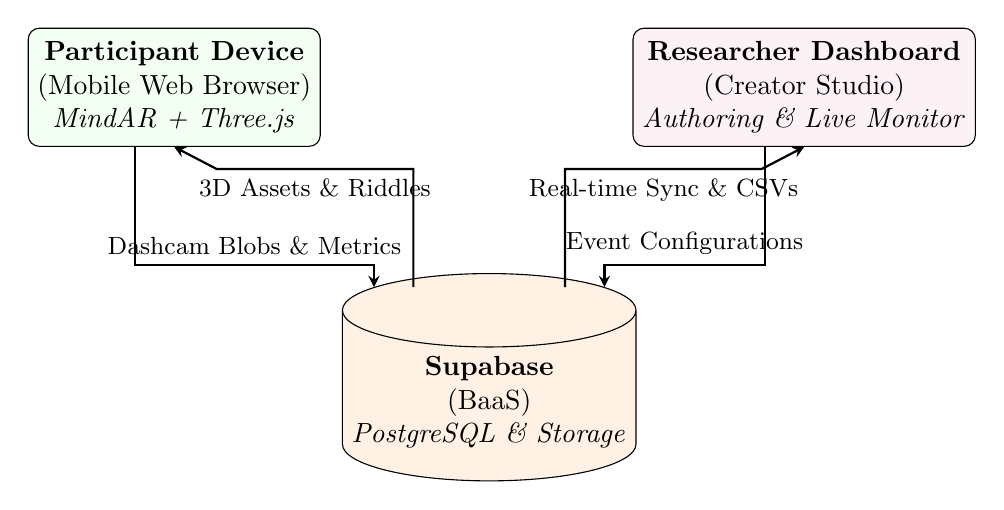
\begin{tikzpicture}[
  box/.style={draw, rounded corners, minimum width=3cm, minimum height=1.5cm, align=center, fill=blue!5},
  db/.style={draw, cylinder, shape border rotate=90, aspect=0.25, minimum width=2.5cm, minimum height=2cm, align=center, fill=orange!10},
  arrow/.style={->, thick, >=stealth}
]

% Nodes
\node[box, fill=green!5] (client) at (0, 0) {\textbf{Participant Device}\\(Mobile Web Browser)\\ \textit{MindAR + Three.js}};
\node[box, fill=purple!5] (admin) at (8, 0) {\textbf{Researcher Dashboard}\\(Creator Studio)\\ \textit{Authoring \& Live Monitor}};
\node[db] (supabase) at (4, -4) {\textbf{Supabase}\\(BaaS)\\ \textit{PostgreSQL \& Storage}};

% Arrows
\draw[arrow] (client.south) ++(-0.5,0) -- ++(0,-1.5) -| node[pos=0.25, above, font=\small] {Dashcam Blobs \& Metrics} (supabase.north west);
\draw[arrow] (supabase.north west) ++(0.5,0) |- node[pos=0.75, below, font=\small] {3D Assets \& Riddles} ++(-2.5,1.5) -- (client.south);

\draw[arrow] (admin.south) ++(-0.5,0) -- ++(0,-1.5) -| node[pos=0.25, above, font=\small] {Event Configurations} (supabase.north east);
\draw[arrow] (supabase.north east) ++(-0.5,0) |- node[pos=0.75, below, font=\small] {Real-time Sync \& CSVs} ++(2.5,1.5) -- (admin.south);

\end{tikzpicture}
}
\caption{The high-level serverless architecture of ARTHunt, demonstrating the real-time data flow between the participant's WebAR interface, the Supabase backend, and the researcher's analytical dashboard.}
\label{fig:architecture}
\end{figure}

\subsection{Software Functionalities}
The platform provides a holistic ecosystem divided into two interfaces:

\begin{itemize}
    \item \textbf{Dynamic Authoring:} Researchers upload 2D target images and define sequential narrative riddles. The system autonomously compiles tracking files within the browser.
    \item \textbf{Silent Dashcam Spatial Tracking:} Upon marker detection, the engine silently captures a composite image appending a millisecond timestamp, allowing researchers to mathematically calculate spatial traversal duration.
    \item \textbf{Live Event Monitor:} A real-time command center featuring a dynamic photo grid for asynchronous observation.
    \item \textbf{Academic Data Exporter:} A one-click CSV generation utility calculating exact spatial tracking durations and UX survey scores for SPSS/R ingestion.
\end{itemize}

\section{Illustrative Examples}
\label{sec:examples}
To demonstrate the utility of the automated data-collection apparatus, a mock deployment involving three participants was executed. Participants navigated a physical space to locate sequential augmented reality markers. The Academic Data Exporter aggregates these behavioral metrics into a structured format (Table \ref{table:csv}), immediately prepared for quantitative statistical analysis such as ANOVA.

\begin{figure}[h]
\centering

\includegraphics[width=0.8\textwidth]{figures/dashboard.png}
\caption{The Creator Dashboard, allowing researchers to dynamically author sequential WebAR events and review spatial traversal metrics.}
\label{fig:dashboard}
\end{figure}

\begin{table}[h]
\centering
\resizebox{\textwidth}{!}{
\begin{tabular}{@{}lccccc@{}}
\toprule
\textbf{Participant ID} & \textbf{Total Duration (ms)} & \textbf{Hints Used} & \textbf{Dashcams} & \textbf{Time to M1 (ms)} & \textbf{Time to M2 (ms)} \\ \midrule
Hunter\_Alpha       & 145,203 & 0 & 2 & 45,102 & 100,101 \\
Hunter\_Beta        & 210,405 & 2 & 2 & 89,000 & 121,405 \\
Hunter\_Gamma       & 112,890 & 0 & 2 & 30,500 & 82,390  \\ \bottomrule
\end{tabular}
}
\caption{Simulated output from the ARTHunt Academic Exporter. The system passively tracks the exact millisecond duration between physical marker discoveries, alongside cognitive load metrics (Hints Used) and verification photographs (Dashcams).}
\label{table:csv}
\end{table}

\section{Impact}
\label{sec:impact}
ARTHunt lowers the barrier to entry for behavioral and educational researchers wishing to conduct pervasive studies. By eliminating the necessity for custom app development, it allows scientists to gather highly accurate spatial traversal data seamlessly in the background.

\section{Conclusions}
\label{sec:conclusions}
ARTHunt successfully bridges the gap between advanced computer vision technologies and accessible behavioral research methodologies, providing a highly rigorous apparatus for scientific inquiry in ubiquitous computing.

\section*{Conflict of Interest}
We wish to confirm that there are no known conflicts of interest associated with this publication.

\section*{Acknowledgements}
The author would like to acknowledge NITK for their continued support.

\bibliography{references}

\end{document}
